\documentclass[a4paper]{article}
\usepackage[affil-it]{authblk}
\usepackage[backend=bibtex,style=numeric]{biblatex}
\usepackage{ctex}
\usepackage{graphicx}
\usepackage{subcaption}
\usepackage{float} 
\usepackage{xcolor}
\usepackage{amsmath}
\usepackage{geometry}
\usepackage{amssymb}
\usepackage{mathtools}
\usepackage{geometry}
\usepackage{listings}
\usepackage{tcolorbox}  % 用于创建带背景的文本框
\usepackage{tikz}  
\usepackage{pgfplots}  % 用于绘制图形
\pgfplotsset{compat=1.18}
\geometry{margin=1.5cm, vmargin={0pt,1cm}}
\setlength{\topmargin}{-1cm}
\setlength{\paperheight}{29.7cm}
\setlength{\textheight}{25.3cm}


\lstset{
	language=C++,                     % 设置语言
	basicstyle=\ttfamily\small,        % 字体样式
	keywordstyle=\color{blue},         % 关键字颜色
	commentstyle=\color{gray},         % 注释颜色
	stringstyle=\color{red},           % 字符串颜色
	numbers=left,                      % 行号显示在左侧
	numberstyle=\tiny\color{gray},     % 行号颜色
	stepnumber=1,                      % 每行显示行号
	frame=single,                      % 加框
	breaklines=true,                   % 自动换行
	captionpos=b,                      % 标题位置
	tabsize=4                          % 制表符宽度
}

\addbibresource{citation.bib}

\begin{document}
% =================================================
\title{NA第二次编程作业代码报告}

\author{高凌溪 3210105373
  \thanks{Electronic address: \texttt{3210105373@zju.edu.cn}}}
\affil{(数应2102), Zhejiang University }


\date{Due time: \today}

\maketitle


% ============================================
\section*{I.程序设计思路}
\begin{enumerate}
	\item 为了定义多项式和更好的输出输出Newton法和Hermite法的结果,首先定义了抽象类\lstinline|Polynomial|,其中包含了以下功能:
\begin{lstlisting}
	class Polynomial{
		private:
		vector<double> coefficients={0.0}; //记录多项式系数,按照升幂排列
		int n=0;  //记录最高次数
		public:
		Polynomial(){};
		Polynomial(vector<double> _coefficients):coefficients(_coefficients){
			n=coefficients.size()-1;
		}
		int Degree() const {} 		//返回多项式次数
		Polynomial operator+(const Polynomial &p1 ) const{}	//实现多项式的加法
		Polynomial operator-()const{}  //实现多项式加负号
		Polynomial operator-(const Polynomial &p1){} //实现多项式减法
		Polynomial operator*(const Polynomial &p1)const{} //实现多项式乘法
		double operator()(double(x))const{} //多项式求值
		Polynomial derivative()const{}  //多项式求导
		void print(ostream &out=cout) const{} 	//输出结果到文件,输出格式为a+bx+...
        void printforpy(ostream &out=cout) const{}//输出结果到文件,输出格式为系数按幂从低到高排列,便于python作图
	};
\end{lstlisting}
	\item
	为了解决A,B,C,D,E,需要实现Newton插值法和Hermite插值法。为了实现Newton插值法和Hermite插值法,我设计了抽象基类\lstinline|Interpolation|,从中继承了\lstinline|Newtoninterpolation|和\lstinline|Hermiteinterpolation|,这个抽象基类实现了以下几个功能:
\begin{lstlisting}
	class Interpolation
	{
		protected:
		vector<double> x, y;  //x 用于存储给定的插值点,y用于存储在给定点上的函数值
		int k=0; //k表示插值点个数
		vector<vector<double>> table; //记录差商表
		public:
		virtual void settable()=0; //构造差商表
		virtual Polynomial  getpolynomial()=0; //最终返回多项式
		vector<vector<double>> gettable(){
			settable();
			return table;
		}
		void print(){}    	//打印差商表
		virtual ~Interpolation()=default; 
	};
\end{lstlisting}
	其中,差商表的具体构造方法完全参考了讲义中的方法。
	\item 
	为了解决F题,参考算法2.74,使用极坐标参数化点的坐标,$x(t)=\sqrt{3}\cos t$,$y(t)=\frac{2}{3}(\sqrt{3}\sin t +\sqrt{|x|})$,然后分别生成$x\: y$关于$t$的多项式。为了对参数求导更方便,使用了数值导数。观察得到曲线上的点仅在横坐标为0时不是$C^1$的,只要取点时避开即可。具体如下:
	\begin{lstlisting}
		class Function {
			public:
			virtual double operator() (double x) const = 0;
			virtual double derivative(double x) const {
				double h=1e-6;
				return ((*this)(x+h)-(*this)(x))/h;
			}
		};
	\begin{lstlisting}
		class Curve{
			protected:
			const Function &F;  //F代表x(t) y(t)的具体表达式
			private:
			vector<double> x={0.0};  //记录取的点pj的坐标
			public:
			Curve(const Function &F, vector<double>x):F(F),x(x){}
			vector<double> Cubic_Bezier(const vector<double> &_v){} 
			//根据输入的点生成控制点
			
			Polynomial get_piecewise_curve(){} //生成每一段的bezier曲线
		};
		
		//在曲线上取点,我使用的取点方法是均匀的取点
		vector<double> Get_points(int n){
			double step =2*pi/n;
			vector<double>v(n+1);
			for(int i=0; i<=n; ++i){
				v[i]=i*step;
			}
			return v;
		};
		void save(int n){};将不同取点数目的结果写入不同的文件夹中
	\end{lstlisting}
\end{enumerate}
\section*{II.运行结果}
F的图像结果为output文件夹中的F.png。
\subsection*{B}
\begin{tcolorbox}[colback=gray!10, colframe=gray!80!black]
	\( n=2 \) 插值多项式 \( p(x) \): \\
	\( 1x^0 - 0.0384615x^2 \) \\
	\( n=4 \) 时插值多项式 \( p(x) \): \\
	\( 1x^0 - 0.171088x^2 + 0.00530504x^4 \) \\
	\( n=6 \) 插值多项式 \( p(x) \): \\
	\( 1x^0 - 0.351364x^2 + 0.0335319x^4 - 0.000840633x^6 \) \\
	\( n=8 \) 插值多项式 \( p(x) \): \\
	\( 1x^0 - 0.528121x^2 + 0.0981875x^4 - 0.00658016x^6 + 0.000137445x^8 \) \\
\end{tcolorbox}

\begin{tikzpicture}
	\begin{axis}[
		xlabel={$x$},
		ylabel={$p(x)$},
		legend pos=north west,
		grid=major,
		width=12cm,
		height=8cm,
		samples=100,
		domain=-5:5
		]
		\addplot[black, thick] {1/(1+x^2)};
		\addlegendentry{原函数}
		% n=2 插值多项式
		\addplot[blue, thick] {1 - 0.0384615*x^2};
		\addlegendentry{$n=2$}
		
		% n=4 插值多项式
		\addplot[red, thick] {1 - 0.171088*x^2 + 0.00530504*x^4};
		\addlegendentry{$n=4$}
		
		% n=6 插值多项式
		\addplot[green, thick] {1 - 0.351364*x^2 + 0.0335319*x^4 - 0.000840633*x^6};
		\addlegendentry{$n=6$}
		
		% n=8 插值多项式
		\addplot[purple, thick] {1 - 0.528121*x^2 + 0.0981875*x^4 - 0.00658016*x^6 + 0.000137445*x^8};
		\addlegendentry{$n=8$}
		
	\end{axis}
\end{tikzpicture}

\subsection*{C}
\begin{tcolorbox}[colback=gray!10, colframe=gray!80!black]
	\( 1x^0 - 3.54298x^2 + 2.7465x^4 \) \\
	\( 0.730822x^0 - 4.81162x^2 + 12.6193x^4 - 14.0024x^6 + 5.51277x^8 \) \\
	\( 1x^0 - 17.3641x^2 + 149.027x^4 - 646.864x^6 + 1510.61x^8 - 1927.18x^{10} + 1264.42x^{12} - 333.619x^{14} \) \\
	\( 0.96241x^0 - 16.5422x^2 + 165.458x^4 - 960.825x^6 + 3379.02x^8 - 7413.45x^{10} + 10195.5x^{12} - 8534.89x^{14} + 3973.16x^{16} - 788.326x^{18} \) \\
\end{tcolorbox}

\begin{tikzpicture}
	\begin{axis}[
		xlabel={$x$},
		ylabel={$p(x)$},
		legend pos=north west,
		grid=major,
		width=12cm,
		height=8cm,
		samples=100,
		domain=-1:1
		]
		\addplot[black, thick] {1/(1+25*x^2)};
		\addlegendentry{原函数}
		% 多项式1
		\addplot[blue, thick] {1 - 3.54298*x^2 + 2.7465*x^4};
		\addlegendentry{$n=5$}
		
		% 多项式2
		\addplot[red, thick] {0.730822 - 4.81162*x^2 + 12.6193*x^4 - 14.0024*x^6 + 5.51277*x^8};
		\addlegendentry{$n=10$}
		
		% 多项式3
		\addplot[green, thick] {1 - 17.3641*x^2 + 149.027*x^4 - 646.864*x^6 + 1510.61*x^8 - 1927.18*x^10 + 1264.42*x^12 - 333.619*x^14};
		\addlegendentry{$n=15$}
		
		% 多项式4
		\addplot[purple, thick] {0.96241 - 16.5422*x^2 + 165.458*x^4 - 960.825*x^6 + 3379.02*x^8 - 7413.45*x^10 + 10195.5*x^12 - 8534.89*x^14 + 3973.16*x^16 - 788.326*x^18};
		\addlegendentry{$n=20$}
		
	\end{axis}
\end{tikzpicture}

\subsection*{D}
\begin{tcolorbox}[colback=gray!10, colframe=gray!80!black]
	displacement(t=10 s)= 742.503 \\
	velocity(t=10 s) = 48.3817\\
	在0~13秒内,速度(feet/second)的函数大致为:
	$75x^0+14.3238x^1-30.2859x^2+22.0325x^3-7.69148x^4+1.45825x^5-0.15313x^6+0.00832472x^7-0.000182013x^8$\\
	由图像很容易看出已经超过81feet/second
\end{tcolorbox}
\begin{tikzpicture}
	\begin{axis}[
		xlabel={$x$},
		ylabel={$p(x)$},
		legend pos=north west,
		grid=major,
		width=12cm,
		height=8cm,
		samples=100,
		domain=0:13
		]

		\addplot [thick,blue]
		{75 + 14.3238*x - 30.2859*x^2 + 22.0325*x^3 - 7.69148*x^4 + 1.45825*x^5 - 0.15313*x^6 + 0.00832472*x^7 - 0.000182013*x^8};
	\end{axis}
\end{tikzpicture}

\subsection*{E}

\begin{tcolorbox}[colback=gray!10, colframe=gray!80!black]
	\( 6.67x^0 - 43.0127x^1 + 16.2855x^2 - 2.11512x^3 + 0.128281x^4 - 0.00371557x^5 + 4.1477 \times 10^{-5} x^6 \) \\
	\( 6.67x^0 - 5.85018x^1 + 2.98227x^2 - 0.424283x^3 + 0.0265858x^4 - 0.000777473x^5 +8.6768\times 10^{-6}x^6\) \\
	14640.3\\
	2981.48	
\end{tcolorbox}

\begin{tikzpicture}
	\begin{axis}[
		xlabel={$x$},
		ylabel={$p(x)$},
		legend pos=north west,
		grid=major,
		width=12cm,
		height=8cm,
		samples=100,
		domain=0:28
		]
		
		% 第一个多项式
		\addplot[blue, thick] {6.67 - 43.0127*x + 16.2855*x^2 - 2.11512*x^3 + 0.128281*x^4 - 0.00371557*x^5 + 4.1477e-5*x^6};
		\addlegendentry{sp1}
		
		% 第二个多项式
		\addplot[red, thick] {6.67 - 5.85018*x + 2.98227*x^2 - 0.424283*x^3 + 0.0265858*x^4 - 0.000777473*x^5+8.6768e-6*x^6};
		\addlegendentry{sp2}
		
	\end{axis}
\end{tikzpicture}

\begin{tikzpicture}
	\begin{axis}[
		xlabel={$x$},
		ylabel={$p(x)$},
		legend pos=north west,
		grid=major,
		width=12cm,
		height=8cm,
		samples=100,
		domain=0:43
		]
		
		% 第一个多项式
		\addplot[blue, thick] {6.67 - 43.0127*x + 16.2855*x^2 - 2.11512*x^3 + 0.128281*x^4 - 0.00371557*x^5 + 4.1477e-5*x^6};
		\addlegendentry{sp1}
		
		% 第二个多项式
		\addplot[red, thick] {6.67 - 5.85018*x + 2.98227*x^2 - 0.424283*x^3 + 0.0265858*x^4 - 0.000777473*x^5+8.6768e-6*x^6};
		\addlegendentry{sp2}
		
	\end{axis}
\end{tikzpicture}
\subsection*{F}
用python作图后得到结果如下:
\begin{figure}[H]  % 使用b选项确保图片在页面底部
	\centering
	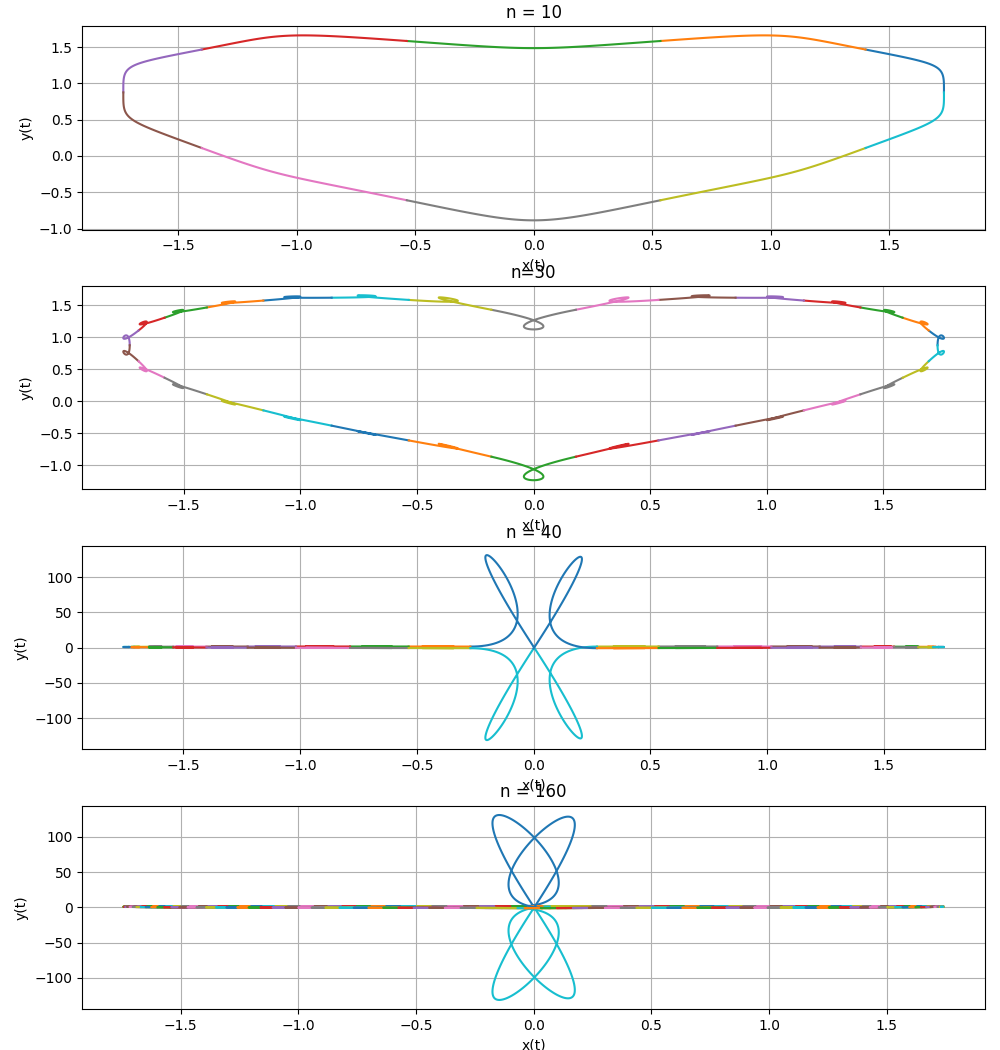
\includegraphics[width=0.5\textwidth]{F.png}  % 调整图片宽度
	\caption{Plot of F}
\end{figure}
\section*{III.结果分析}
\subsection*{B C}
首先从B C的结果不难发现,当原函数是一个偶函数且取的插值点是关于$y$轴对称时,用Newton插值得到的插值多项式也是一个偶函数。\\
从B的结果可以看出,即使插值点变多,插值多项式的拟合效果也只是在区间$[-2,2]$上变好,但是在靠近$-5$和$5$的位置,会出现剧烈的震荡,一致误差反而随之插值点的增多而增大。\\
C中的结果展示了第一类切比雪夫多项式可以更好的拟合$\frac{1}{1+25x^2}$这个函数,在插值点数目为20的时候,从图像上看拟合效果已经很好,插值多项式虽然仍然在靠近$-1$和$1$的部分有一定的震荡,但是误差的一致范数已经可以被控制住并且不大。\\
\subsection*{E}
E中的结果显然与显示不符,事实上作出E中的插值多项式图像可以看到,插值多项式在区间$[28,43]$上迅速增长,根据讲义定理2.7插值多项式的误差$R_n(f;x)=\frac{f^{(n+1)}(\xi)}{(n+1)!}\prod_{i=0}^{n}(x-x_i) $,带入这个公式可以发现当$x$很大时,误差也会很大,因此使用插值多项式预测$x=43$时,$f(x)$的值并不合理,应该使用其他方法。

\subsection*{F}
通过用python作图可以发现,在使用角度作为参数的时候,在$[0,2\pi]$上均匀的取点生成控制点并不是一个好的方式。在取点数$n$比较小的时候,bezier曲线不会自交,拟合效果一般,但$n$很大时,曲线自交会非常严重,无法拟合曲线。按照我取点的方式,我认为拟合效果最好的是$n=30$的情况。\\
分析:曲线自交的原因是由于在$p_j$和$p_{j+1}$处的切线模长太大。假设$x(t)=\sqrt{3}\cos t$,$y(t)=\frac{2}{3}(\sqrt{3}\sin t +\sqrt{|x|})$,求导得到${x}'(t)=-\sqrt{3}\sin t$,${y}'(t)=\frac{2}{3}(\sqrt{3}\cos t+\frac{-\sqrt{3}\sin t}{2\sqrt{\sqrt{3} \cos t}})$,从导数可以看出,当$t \to \frac{\pi}{2}$时,切线的模长会非常大,这也能解释$n=160$时图像产生的原因。因此在取点的时候应该避开$y$轴附近的点。而通过观察$n=30$的图像可以发现,几乎每一段bezier曲线都有自相交的情况,因此我认为这个图形并不适合用三次bezier曲线分段拟合。
% ===============================================
\section*{ \center{\normalsize {Acknowledgement}} }
Give your acknowledgements here(if any).


\printbibliography

If you are not familiar with \texttt{bibtex}, 
it is acceptable to put a table here for your references.
\end{document}
